\chapter{Methodology}
\section{Kernel Selection}
So that a breadth of usage scenarios were examined, three kernels were selected based on their conformity to the following set of criteria.
\begin{itemize}
  \item \textbf{The part of the program responsible for more than two thirds of the processing time should not be more than 1500 lines.} To ensure that I fully implemented three ports of existing kernels, it was necessary to limit the size of the kernels that could be considered. This was an unfortunately necessary decision to make. Whilst it reduced the field of possible kernels, it helpfully excluded any overly complex mini-apps.

  \item \textbf{The program must use shared memory parallelism and target the CPU.} Rust's (supposed) zero cost memory safety features are its differentiating factor. The best way to test the true cost of Rust's memory safety features would be through shared memory parallelism, where a poor implementation of memory management will make itself evident through poor performance. Programs which target the GPU rather than the CPU will not be considered, as the current implementations for Rust to target GPUs involve calling out to existing GPU APIs. Therefore, any analysis of a Rust program targeting a GPU would largely be an analysis of the GPU API itself.

  \item \textbf{The program run time should reasonably decrease as the number of threads increases, at least until the number of threads reaches 32.} It is important that any kernel considered is capable of scaling to the high core counts normally seen in HPC.I will be running the kernels on Cirrus, which supports 36 real threads.

  \item \textbf{The program operate on data greater than the CPU's L3 Cache} so that we can be sure that the kernel is representative of working on large data sets. Cirrus has an L3 cache of 45MiB. As each node has 256GB of RAM, a central constraint when working with large data sets is the speed with which data is loaded into the cache. Speed is often achieved by programs in this area through vectorisation, the use of which can be deduced from a program's assembly code. If there is a large performance difference between Rust and the reference kernels, we can use the program's assembly code to reason about that difference.

  \item \textbf{The program must be written in C or C++.} This restriction allows us to choose work which is more representative of HPC programs that actually run on HPC systems, rather than python programs which call out to pre-compiled libraries. Unlike Fortran, C and C++ use array indexing and layout conventions similar to Rust, which will make porting programs from them easier.

  \item \textbf{The program must use OMP.} This is a typical approach for shared memory parallelism in HPC. Use of a library to do the parallel processing also further standardises the candidate programs, which will lead to a deeper understanding of the kernel's performance factors.
\end{itemize}

I used this selection criteria to compile a long list of potential kernels to port to Rust. From this long list, I selected the Babel Stream, sparse matrix vector multiplication and K-means clustering.

\subsection{Babel Stream}

Babel Stream is a memory bench marking tool which was developed by the university of Bristol. Babel Stream was written to primarily target GPUs, but it is able to target CPUs too~\cite{BabelStream}.  It is written in C++, supports OpenMP and allows one to set the problem size when executing the program, so we can be sure we exceed the size of L3 cache. Tests found the kernel to scale well, and although the program as a whole is quite large, when one ignores parallel technologies excluded by our selection criteria, the amount of code which needs to be ported to Rust falls well within our bounds.

Babel Stream performs simple operations on three arrays of either 32 or 64 bit floating point numbers, $a$, $b$ and $c$. The values of $a$ are set to 0.1, $b$'s to 0.2, and $c$'s to 0.0. Stream performs five operations $n$ times on the arrays, where $n$ is a specified command line argument. The operations are listed below:
\begin{itemize}
  \item \textbf{Copy:} Data is copied from the array $a$ into array $c$
  \item \textbf{Multiply:} Data in $c$ is multiplied by a scalar and stored in $b$
  \item \textbf{Add:} The values in $a$ and $b$ are added together and stored in $c$
  \item \textbf{Triad:} The program then multiplies the new values in $c$ by the same scalar value, adds it to $b$ and stores the value in $a$
  \item \textbf{Dot:} The dot product is performed on arrays $a$ and $b$. This is when every nth element of $a$ is multiplied by the nth element of $b$, and summed.
\end{itemize}
The resulting values in the arrays are then compared against separately calculated reference values, and examined to see if their average error is greater than that number types epsilon value.

Babel Stream's simple mathematical operations provide an insight into the memory bandwidth of a programming language, and give an indication of how the  design choices of a language can influence their performance.

\subsection{Sparse}

The Sparse Kernel~\cite{ParResSparse} forms part of the Parallel Research Kernels suite, developed by the Parallel Research Tools group. Sparse matrix vector multiplication is a common HPC operation, used to solve a broad range of scientific problems~\cite{Sedaghati:2015, spMVGPU, DBLP:journals}.

The kernel mostly one file, sparse.c, which in total is 353 lines of code. The implementation is in C and OpenMP, and tests found it to scale to a high thread count. As with Babel Stream, the program allows one to set problem size through command line arguments, allowing us to ensure the program operated on data greater than the CPU's L3 cache.

The program represents its sparse matrix through the compressed sparse row (CSR) format. This format uses key information about the matrix to avoid storing all of the sparse matrix's redundant zeros in the computer's memory. The information used to do this are the number of rows and columns the matrix has, and the number of non zero values which exist in the matrix. These three values are used to build three vectors, one holding all the non zero values of the matrix, another vector of the same length holding the column indexes for all of those values, in order, and lastly a smaller vector which holds the index at which a particular row starts. For example, if we wanted the element at 24,32 within the vector, we would look in the 24\textsuperscript{th} element of the row start vector, which would give us the y index of the element. If this did not match the y index we were looking for, in this case 32, we would then look at the next element until we found it. Once we have found the element, we can get the value from the value vector using the index we construct from adding the 24\textsuperscript{th} element of the row start vector, added to however many times we needed to look at the next value to before we found the appropriate y index.

The particular implementation of sparse matrix vector multiplication which we are porting to Rust uses a user defined grid size, over which a user defined periodic stencil is applied to find the number of non zero entries. The implementation parallelises its initialisation and the actual multiplication of the values using simple \texttt{\#pragma} statements.

This kernel will hopefully provide a realistic idea of how well Rust can perform one of the most common HPC operations.

\subsection{K Means}

K means is common etc, this implementation also uses netcdf which is also v common so interesting to see how hard it is to get Rust to work with it.

\section{Implementation}
Implementation of all three programs follows the same process, as outlined in Figure~\ref{fig:imp-flow}. The full process would take between three to four weeks to complete for each kernel. I first implemented Babel Stream, then the sparse matrix multiplication kernel and finally the K means kernel in that order.

\begin{figure}
  \center
  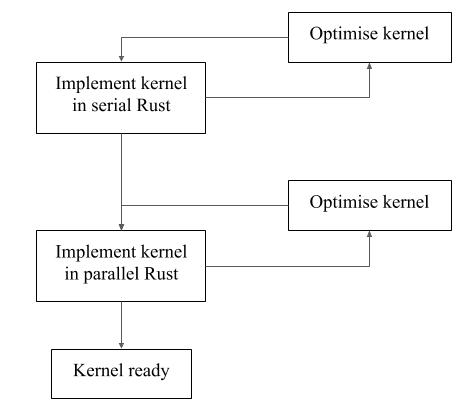
\includegraphics[height=12cm]{figs/ImplementationFlow.png}
  \caption{Flow Diagram for Implementation Process}
  \label{fig:imp-flow}
\end{figure}

\subsection{Porting to Serial Rust}
Once a candidate kernel is selected, it is implemented in Rust in serial. Any differences between the  behaviour of the Rust and the original implementation are thought of as bugs, and are eradicated or minimised as far as is possible. For ease of development, the Rust crate Clap was used to read command line arguments for the program, leading to Rust implementations of kernels being called with slightly different syntax. This difference was deemed to be superficial enough to be allowable. Kernel output was ensured to be as similar as possible to aid data-collection from both implementations.

Babel Stream was in some ways one of the hardest to Kernels to port to serial Rust. This was partly due to it being the first program which I attempted to port, but also because of Rusts type system and the use of generics. The original C++ implementation of the program uses templates to allow the user to choose to use 32 or 64 bit floating numbers when running the program. To achieve the same thing in Rust, generics types have to be used, which are defined through traits. This made reading error messages slightly difficult, but easier to parse once the offending code was removed into a smaller example, and stripped of its generic type. Generics in Rust also necessitate the slightly cumbersome syntax \texttt{T::from(0).unwrap()} to generate a zero of type T. This expression generates an option type, which in this case is \texttt{Some(0.0)}, and is then unwrapped into simply \texttt{0}. Rust does this to allow programmers to deal with cases where a value of type T is impossible to generate from the input value, as casting a value greater than $2^{32} - 1$ to a signed 32 bit value. In this circumstance, the value returned would be \texttt{None}, which the programmer would then have to deal with. As zero can always be successfully cast to a 32 or 64 bit floating point number, it is safe to simply unwrap the value here, but if it was a number that could not be cast to the type, then the program would crash at this point.

The Rust implementation of Babel stream, like the reference implementation, creates a stream object which calls certain functions on its own data sets. This was quite easy to implement as Rust has enough features of object oriented design, such as allowing objects to contain data and behaviour for these simple objects to work. However, Rust does not implement inheritance, which is conisdered by some to be a foundational aspect of object oriented programming~\cite{Liskov:1987}, and instead uses trait objects to share behaviours. This design choice did not interfere with any of the simple kernels which were implemented, but would certainly be interesting to translate object inheritance from a larger program, maybe a mini-app, into Rust's trait objects.

Whilst the concept of borrowing did take some time to fully understand, I found that the compiler gave very helpful and accurate hints on how to make sure my program complied with the borrow checker. For example, in listing~\ref{lst:comp-help}, the programmer is informed that they ``cannot borrow self.c as mutable'', and is shown where the function tries to mutate the value. The stream object's triad function, which alters the objects data, but take mutable ownership of the data, through using \texttt{\&mut self}, where \texttt{\&mut} is a mutable borrow. Once the programmer implements the compiler's suggested fix, this fragment of code will compile.

\begin{lstlisting}[language=Rust,label=lst:comp-help,caption=Help from the Rust compiler]
error[E0596]: cannot borrow `self.c` as mutable, as it is behind a
              `&` reference
  --> src/stream.rs:20:9
   |
18 |     pub fn triad(&self){
   |                  ----- help: consider changing this to be a
    mutable reference: `&mut self`
20 |         self.c[0] = self.a[0] + self.b[0];
   |         ^^^^^^ `self` is a `&` reference, so the data it refers
    to cannot be borrowed as mutable

error: aborting due to previous error
\end{lstlisting}

The sparse matrix vector multiplication kernel was quite simple to port to serial Rust, as I was able to ignore parts of the small program which would not be used. As with Babel Stream, I found converting from C's data types into Rust to be a stumbling point due to Rust's safety constraints. For example, in the C implementation, the vector holding the column index of the matrix was composed of values of type \texttt{s64Int}, which a signed 64 bit int. This datatype is directly analogous to Rust's \texttt{i64} data type, except in C you may use numbers of type \texttt{s64Int} to index into arrays, where as in Rust you must only use numbers of type \texttt{usize}. Errors of this type are easily dealt with however, as they are explicitly pointed out to the programmer at compile time, and can be remedied with casts in the simple format \texttt{as usize}. I found sparse matrix vector multiplication easier to port to serial Rust than Babel Stream, but this could have been that by this point I was already more familiar with Rust's way of doing things.

some stuff about K means, how easy it was to get netcdf working because of cargo

\subsection{Bug fixing, conversion to idiomatic Rust}
Next, I would eliminate any bugs found in my serial implementation of the code by comparing outputs between my implementation and the reference implementation. During this process I would also move the code away from its C conventions towards more idiomatic Rust. To achieve more idiomatic Rust, I used the linting tool Clippy~\cite{RustClippy}, which was developed by the Rust team.  Clippy includes a category of lints under  which highlight `code that should be written in a more idiomatic way'~\cite{RustClippy}. I implemented all of Clippy's recommended rewrites, which would often include replacing the use of for loops to access vector variables with calls to the vectors \texttt{iter()} method. This particular replacement could require code to be rewritten in a much more functional style.

For example, all of the array operations in Babel Stream where originally written in a C style, and then transformed to use iterators. Listing~\ref{lst:iters-b}, shows the original, more succint for of Babel Stream's add operation. This style is rejected by Clippy, which prefers the style presented by listing~\ref{lst:iters-a}.
\begin{lstlisting}[language=Rust, label=lst:iters-b, caption={Babel Stream Add, before applying idomatic Rust style}]
for i in 0..self.c.len() as usize {
    self.c[i] = self.b[i] + self.a[i]
}
\end{lstlisting}
Whilst the more idiomatic rust style in listing~\ref{lst:iters-a} is less succint than~\ref{lst:iters-b}, it does have some benefits which does not posses. For example, if the stream object's c array had been of greater length than its $a$ or $b$ arrays, the more C like implementation would fail at run time withan index out of bounds error, where as the more Rustic code only write to as many elements of $c$ as the least elements there are of any of the arrays it is zipped with.
\begin{lstlisting}[language=Rust, label=lst:iters-a, caption={Babel Stream Add, after applying idomatic Rust style}]
for ((c, b), a) in self.c.iter_mut()
                         .zip(self.b.iter())
                         .zip(self.a.iter()){
    *c = *b + *a;
}
\end{lstlisting}
Also note in listing~\ref{lst:iters-a} the distinction between the methods \texttt{iter()} and \texttt{iter\_mut()}, the first of which create an iterator, and the second of which creates an iterator which may change its elements. Although an indepth investigation was not carried out to see if the compiler made use of any optimisations here from the greater amount of information available to it, the time to run this fragment did decrese when converted to idiomatic Rust, from 0.09501 seconds to 0.09079 seconds.

A bug in the SpMV implementation made itself apparent when I noticed that when launched with certain parameters, the C version ran without error, whilst the Rust version would panic and fail every time, with the error message:

thread 'main' panicked at 'attempt to shift left with overflow', main.rs:8:13

It became apparent that this was occuring because although I had mirrored the types used by the reference implementation, the behaviour of those types differed. In the reference implementation, radius was of type \texttt{int}, which is a 32-bit integer. I therefore translated this into a \texttt{i32} type in Rust. These values are used as upper limits in an initilisation loop, where intermediate values of the same type are bit-shifted before being stored in the colIndex array. In C, the operation

  $foo = 1 << 33$

sets $foo$ to 2, when all numbers are 32 bit integers. This occurs because the value 1 overflows and rolls over. In Rust however, this code causes the program to panic and quit~\footnote{The compiler will catch this error before run time if it can calculate the value 1 will be shifted by}. The Rust language does not consider this behavior to be unsafe, but finds that that the programmer `should' find it `undesirable, unexpected or unsafe'~\cite{rustunsafe}. However, Rust does recognise that some programs do rely upon overflow arithmatic, and provides mechanisms to enable this feature in the language. Fortunately, I was not required to use this feature by instead changing radius from the \texttt{i32} type to \texttt{usize} type, which is 64 bits. This choice was made because the radius values were being cast to \texttt{usize} more often than they were being used as \texttt{i32}. This had the consequence of making the program impossible to bit shift overflow, as a radius of 64 requires a stencil diameter greater than $2^{32}-1$, which would in turn require a colindex array terrabytes in size, which the Cirrus hardware does not support.

Clippy was dumb with a loop in K-means, telling me to replace
\begin{lstlisting}[language=Rust]
for k in 1..clusters_d.len as usize {
\end{lstlisting}
with
\begin{lstlisting}[language=Rust]
 for (k, <item>) in old_cluster_centres.iter().enumerate().take(clusters_d.len as usize).skip(1) {
\end{lstlisting}
which really shows the limits of it as a tool to make Rust idiomatic, or how blindly following rules to get idiomatic code can make things worse
\subsection{Parallelisation}
I would then parallelise the kernel using Rayon~\cite{RustRayon} at the same loops where the reference implementation used OpenMP to parallelise its loops. Sometimes this would be a simple matter of replacing the \texttt{iter()} method with \texttt{par\_iter()}, but parallising more complex operations like reductions and initilisations was slightly more difficult.

Parallelising Babel Stream was simple. As listing~\ref{lst:iters-p} shows, Babel Stream's add operation remains largely the same, only that the \texttt{iter()} method has been replaced by the \texttt{par\_iter()} method, and that the method for each has to be called. As the serial version of this loop had no inter loop dependencies, it coud easily be transformed from a for loop to a for each one.
\begin{lstlisting}[language=Rust, label=lst:iters-p, caption={Babel Stream Add, parallelised}]
self.c.par_iter_mut()
            .zip(self.b.par_iter())
            .zip(self.a.par_iter())
            .for_each(|((c, b), a)| *c = *a + *b);
\end{lstlisting}

Then we did some chunking
\begin{lstlisting}[language=Rust]
self.c.par_chunks_mut(self.chunk_size)
    .zip(self.b.par_chunks(self.chunk_size))
    .zip(self.a.par_chunks(self.chunk_size))
    .for_each(|((c, b), a)|
                    for ((c_i, b_i), a_i) in c.iter_mut()
                                                .zip(b.iter())
                                                .zip(a.iter()){
                                                    *c_i = *a_i + *b_i
                                                });
\end{lstlisting}


\subsection{Debug final implementation}
Once I had parallelised the Rust implementation, I would again debug the program process at this stage could be hard to fix as they could come from original implementations. An interesting example of such a bug is discussed further in this section, from the sparse matrix vector multiplication kernel.

Initialisation is the very verbose - Explain why it's so verbose, process for finding this to be worth doing etc.
\begin{lstlisting}[language=Rust]
vec![0.0; arr_size].par_iter()
                   .map(|_| T::from(0.2).unwrap())
                   .collect_into_vec(&mut self.b);
\end{lstlisting}

Talk about finding horrendus parallel init bug in Sparse

Once the implementation process had been finished, testing could begin.

\subsubsection{Babel Stream}
\begin{itemize}
  \item Type problems due to generics leading to verbose code and obfuscating debugging
  \item The compiler did help with type debugging a little, but had limitations - give example
  \item Idiomatic serial Rust was faster than C like rust, potentially due to iter\_mut allowing optimisations? Evidence from triad and add.
  \item Once I figured out the for\_each pattern is was easy to apply it to other operations
  \item Realised that Rust's serial init was a bottleneck
  \item difficulty in writing para init as not a common use case scenario, and obfuscated by type
\end{itemize}








\subsubsection{Sparse Matrix}
\begin{itemize}
  \item Bit shift overflow causes Rust to crash not just run on, have to be more careful about kernel input parameters. Initially thought this might be a bug. Give example.
  \item Found init bug, was very difficult to implement para init. Filed bug report with original project
  \item remember that class you tried to build to increment stuff? m8
\end{itemize}

\subsection{Experimentation}

\section{Questionnaire}
